\documentclass[twoside]{book}

% Packages required by doxygen
\usepackage{calc}
\usepackage{doxygen}
\usepackage{graphicx}
\usepackage[utf8]{inputenc}
\usepackage{makeidx}
\usepackage{multicol}
\usepackage{multirow}
\usepackage{textcomp}
\usepackage[table]{xcolor}

% Font selection
\usepackage[T1]{fontenc}
\usepackage{mathptmx}
\usepackage[scaled=.90]{helvet}
\usepackage{courier}
\usepackage{amssymb}
\usepackage{sectsty}
\renewcommand{\familydefault}{\sfdefault}
\allsectionsfont{%
  \fontseries{bc}\selectfont%
  \color{darkgray}%
}
\renewcommand{\DoxyLabelFont}{%
  \fontseries{bc}\selectfont%
  \color{darkgray}%
}

% Page & text layout
\usepackage{geometry}
\geometry{%
  a4paper,%
  top=2.5cm,%
  bottom=2.5cm,%
  left=2.5cm,%
  right=2.5cm%
}
\tolerance=750
\hfuzz=15pt
\hbadness=750
\setlength{\emergencystretch}{15pt}
\setlength{\parindent}{0cm}
\setlength{\parskip}{0.2cm}
\makeatletter
\renewcommand{\paragraph}{%
  \@startsection{paragraph}{4}{0ex}{-1.0ex}{1.0ex}{%
    \normalfont\normalsize\bfseries\SS@parafont%
  }%
}
\renewcommand{\subparagraph}{%
  \@startsection{subparagraph}{5}{0ex}{-1.0ex}{1.0ex}{%
    \normalfont\normalsize\bfseries\SS@subparafont%
  }%
}
\makeatother

% Headers & footers
\usepackage{fancyhdr}
\pagestyle{fancyplain}
\fancyhead[LE]{\fancyplain{}{\bfseries\thepage}}
\fancyhead[CE]{\fancyplain{}{}}
\fancyhead[RE]{\fancyplain{}{\bfseries\leftmark}}
\fancyhead[LO]{\fancyplain{}{\bfseries\rightmark}}
\fancyhead[CO]{\fancyplain{}{}}
\fancyhead[RO]{\fancyplain{}{\bfseries\thepage}}
\fancyfoot[LE]{\fancyplain{}{}}
\fancyfoot[CE]{\fancyplain{}{}}
\fancyfoot[RE]{\fancyplain{}{\bfseries\scriptsize Generated on Thu Jan 4 2018 09\-:35\-:42 for ogls by Doxygen }}
\fancyfoot[LO]{\fancyplain{}{\bfseries\scriptsize Generated on Thu Jan 4 2018 09\-:35\-:42 for ogls by Doxygen }}
\fancyfoot[CO]{\fancyplain{}{}}
\fancyfoot[RO]{\fancyplain{}{}}
\renewcommand{\footrulewidth}{0.4pt}
\renewcommand{\chaptermark}[1]{%
  \markboth{#1}{}%
}
\renewcommand{\sectionmark}[1]{%
  \markright{\thesection\ #1}%
}

% Indices & bibliography
\usepackage{natbib}
\usepackage[titles]{tocloft}
\setcounter{tocdepth}{3}
\setcounter{secnumdepth}{5}
\makeindex

% Hyperlinks (required, but should be loaded last)
\usepackage{ifpdf}
\ifpdf
  \usepackage[pdftex,pagebackref=true]{hyperref}
\else
  \usepackage[ps2pdf,pagebackref=true]{hyperref}
\fi
\hypersetup{%
  colorlinks=true,%
  linkcolor=blue,%
  citecolor=blue,%
  unicode%
}

% Custom commands
\newcommand{\clearemptydoublepage}{%
  \newpage{\pagestyle{empty}\cleardoublepage}%
}


%===== C O N T E N T S =====

\begin{document}

% Titlepage & ToC
\hypersetup{pageanchor=false}
\pagenumbering{roman}
\begin{titlepage}
\vspace*{7cm}
\begin{center}%
{\Large ogls }\\
\vspace*{1cm}
{\large Generated by Doxygen 1.8.6}\\
\vspace*{0.5cm}
{\small Thu Jan 4 2018 09:35:42}\\
\end{center}
\end{titlepage}
\clearemptydoublepage
\tableofcontents
\clearemptydoublepage
\pagenumbering{arabic}
\hypersetup{pageanchor=true}

%--- Begin generated contents ---
\chapter{Hierarchical Index}
\section{Class Hierarchy}
This inheritance list is sorted roughly, but not completely, alphabetically\-:\begin{DoxyCompactList}
\item \contentsline{section}{ogls\-:\-:Color\-R\-G\-B}{\pageref{d4/d4d/structogls_1_1ColorRGB}}{}
\item exception\begin{DoxyCompactList}
\item \contentsline{section}{ogls\-:\-:Program\-Exception}{\pageref{d8/dbf/structogls_1_1ProgramException}}{}
\item \contentsline{section}{ogls\-:\-:Shader\-Exception}{\pageref{d2/d41/structogls_1_1ShaderException}}{}
\end{DoxyCompactList}
\item \contentsline{section}{ogls\-:\-:Program}{\pageref{d6/d07/classogls_1_1Program}}{}
\item \contentsline{section}{ogls\-:\-:Shader}{\pageref{d1/d2c/classogls_1_1Shader}}{}
\begin{DoxyCompactList}
\item \contentsline{section}{ogls\-:\-:Fragment\-Shader}{\pageref{d5/d46/classogls_1_1FragmentShader}}{}
\begin{DoxyCompactList}
\item \contentsline{section}{ogls\-:\-:Solid\-Color\-Shader}{\pageref{d7/d31/classogls_1_1SolidColorShader}}{}
\end{DoxyCompactList}
\item \contentsline{section}{ogls\-:\-:Vertex\-Shader}{\pageref{dd/da1/classogls_1_1VertexShader}}{}
\end{DoxyCompactList}
\end{DoxyCompactList}

\chapter{Class Index}
\section{Class List}
Here are the classes, structs, unions and interfaces with brief descriptions\-:\begin{DoxyCompactList}
\item\contentsline{section}{\hyperlink{structogls_1_1ColorRGB}{ogls\-::\-Color\-R\-G\-B} }{\pageref{d4/d4d/structogls_1_1ColorRGB}}{}
\item\contentsline{section}{\hyperlink{classogls_1_1FragmentShader}{ogls\-::\-Fragment\-Shader} }{\pageref{d5/d46/classogls_1_1FragmentShader}}{}
\item\contentsline{section}{\hyperlink{classogls_1_1Program}{ogls\-::\-Program} }{\pageref{d6/d07/classogls_1_1Program}}{}
\item\contentsline{section}{\hyperlink{structogls_1_1ProgramException}{ogls\-::\-Program\-Exception} }{\pageref{d8/dbf/structogls_1_1ProgramException}}{}
\item\contentsline{section}{\hyperlink{classogls_1_1Shader}{ogls\-::\-Shader} }{\pageref{d1/d2c/classogls_1_1Shader}}{}
\item\contentsline{section}{\hyperlink{structogls_1_1ShaderException}{ogls\-::\-Shader\-Exception} }{\pageref{d2/d41/structogls_1_1ShaderException}}{}
\item\contentsline{section}{\hyperlink{classogls_1_1SolidColorShader}{ogls\-::\-Solid\-Color\-Shader} }{\pageref{d7/d31/classogls_1_1SolidColorShader}}{}
\item\contentsline{section}{\hyperlink{classogls_1_1VertexShader}{ogls\-::\-Vertex\-Shader} }{\pageref{dd/da1/classogls_1_1VertexShader}}{}
\end{DoxyCompactList}

\chapter{Class Documentation}
\hypertarget{structogls_1_1ColorRGB}{\section{ogls\-:\-:Color\-R\-G\-B Struct Reference}
\label{structogls_1_1ColorRGB}\index{ogls\-::\-Color\-R\-G\-B@{ogls\-::\-Color\-R\-G\-B}}
}
\subsection*{Public Member Functions}
\begin{DoxyCompactItemize}
\item 
\hypertarget{structogls_1_1ColorRGB_adda6e4c3d16a5223e4448926cae42e6e}{{\bfseries Color\-R\-G\-B} (G\-Lfloat r, G\-Lfloat g, G\-Lfloat b)}\label{structogls_1_1ColorRGB_adda6e4c3d16a5223e4448926cae42e6e}

\item 
\hypertarget{structogls_1_1ColorRGB_adf308e06c0ffb612ab463729006c08b2}{bool {\bfseries operator==} (const \hyperlink{structogls_1_1ColorRGB}{Color\-R\-G\-B} \&c) const }\label{structogls_1_1ColorRGB_adf308e06c0ffb612ab463729006c08b2}

\end{DoxyCompactItemize}
\subsection*{Public Attributes}
\begin{DoxyCompactItemize}
\item 
\hypertarget{structogls_1_1ColorRGB_abb7530c0981b6cc9cd77bf21bdb595e0}{G\-Lfloat {\bfseries r}}\label{structogls_1_1ColorRGB_abb7530c0981b6cc9cd77bf21bdb595e0}

\item 
\hypertarget{structogls_1_1ColorRGB_a72cbd03e8ec12a3da22261f873c4ec75}{G\-Lfloat {\bfseries g}}\label{structogls_1_1ColorRGB_a72cbd03e8ec12a3da22261f873c4ec75}

\item 
\hypertarget{structogls_1_1ColorRGB_a2925e36d7044e74da5e50a349dc63906}{G\-Lfloat {\bfseries b}}\label{structogls_1_1ColorRGB_a2925e36d7044e74da5e50a349dc63906}

\end{DoxyCompactItemize}


The documentation for this struct was generated from the following file\-:\begin{DoxyCompactItemize}
\item 
include/colors.\-hpp\end{DoxyCompactItemize}

\hypertarget{classogls_1_1FragmentShader}{\section{ogls\-:\-:Fragment\-Shader Class Reference}
\label{classogls_1_1FragmentShader}\index{ogls\-::\-Fragment\-Shader@{ogls\-::\-Fragment\-Shader}}
}


Inheritance diagram for ogls\-:\-:Fragment\-Shader\-:\nopagebreak
\begin{figure}[H]
\begin{center}
\leavevmode
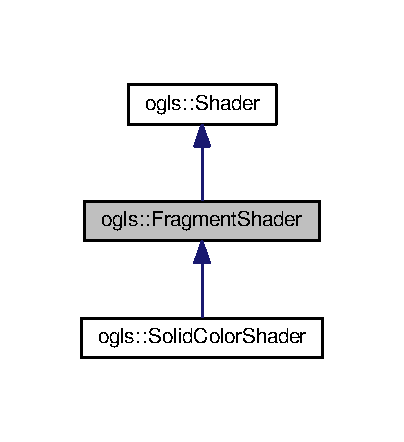
\includegraphics[width=194pt]{d1/d60/classogls_1_1FragmentShader__inherit__graph}
\end{center}
\end{figure}


Collaboration diagram for ogls\-:\-:Fragment\-Shader\-:\nopagebreak
\begin{figure}[H]
\begin{center}
\leavevmode
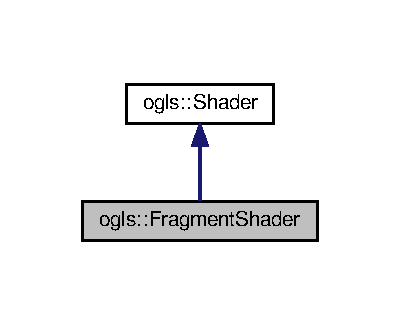
\includegraphics[width=192pt]{d9/d73/classogls_1_1FragmentShader__coll__graph}
\end{center}
\end{figure}
\subsection*{Public Member Functions}
\begin{DoxyCompactItemize}
\item 
\hypertarget{classogls_1_1FragmentShader_aeb28087000e1456f5d31e5857f134644}{{\bfseries Fragment\-Shader} (std\-::string source)}\label{classogls_1_1FragmentShader_aeb28087000e1456f5d31e5857f134644}

\end{DoxyCompactItemize}


The documentation for this class was generated from the following files\-:\begin{DoxyCompactItemize}
\item 
include/shader.\-hpp\item 
src/shader.\-cpp\end{DoxyCompactItemize}

\hypertarget{classogls_1_1Program}{\section{ogls\-:\-:Program Class Reference}
\label{classogls_1_1Program}\index{ogls\-::\-Program@{ogls\-::\-Program}}
}
\subsection*{Public Member Functions}
\begin{DoxyCompactItemize}
\item 
\hypertarget{classogls_1_1Program_a5cddec31b6cb620d64b7024298d20326}{\hyperlink{classogls_1_1Program}{Program} \& {\bfseries add\-Shader} (\hyperlink{classogls_1_1Shader}{Shader} \&shader)}\label{classogls_1_1Program_a5cddec31b6cb620d64b7024298d20326}

\item 
\hypertarget{classogls_1_1Program_ab4baa3dce11c4672e9d3dd97bf94e4b1}{{\footnotesize template$<$typename T $>$ }\\\hyperlink{classogls_1_1Program}{Program} \& {\bfseries set\-Uniform} (const G\-Lchar $\ast$name, std\-::initializer\-\_\-list$<$ T $>$ v)}\label{classogls_1_1Program_ab4baa3dce11c4672e9d3dd97bf94e4b1}

\item 
\hypertarget{classogls_1_1Program_a7d716fc5d669e28aa643affa93e36d67}{\hyperlink{classogls_1_1Program}{Program} \& {\bfseries link} ()}\label{classogls_1_1Program_a7d716fc5d669e28aa643affa93e36d67}

\item 
\hypertarget{classogls_1_1Program_a1438547a0bef924248adb1ebda78656e}{\hyperlink{classogls_1_1Program}{Program} \& {\bfseries use} ()}\label{classogls_1_1Program_a1438547a0bef924248adb1ebda78656e}

\end{DoxyCompactItemize}


The documentation for this class was generated from the following files\-:\begin{DoxyCompactItemize}
\item 
include/program.\-hpp\item 
src/program.\-cpp\end{DoxyCompactItemize}

\hypertarget{structogls_1_1ProgramException}{\section{ogls\-:\-:Program\-Exception Struct Reference}
\label{structogls_1_1ProgramException}\index{ogls\-::\-Program\-Exception@{ogls\-::\-Program\-Exception}}
}


Inheritance diagram for ogls\-:\-:Program\-Exception\-:\nopagebreak
\begin{figure}[H]
\begin{center}
\leavevmode
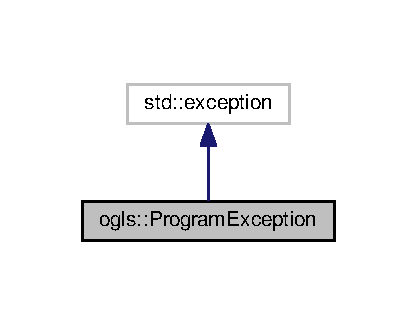
\includegraphics[width=200pt]{d2/d5f/structogls_1_1ProgramException__inherit__graph}
\end{center}
\end{figure}


Collaboration diagram for ogls\-:\-:Program\-Exception\-:\nopagebreak
\begin{figure}[H]
\begin{center}
\leavevmode
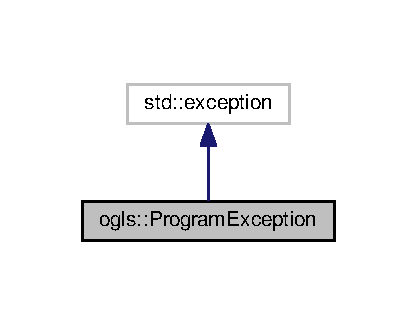
\includegraphics[width=200pt]{d2/d29/structogls_1_1ProgramException__coll__graph}
\end{center}
\end{figure}
\subsection*{Public Member Functions}
\begin{DoxyCompactItemize}
\item 
\hypertarget{structogls_1_1ProgramException_afeaffb31d0feabdc28590e18dbdd13e2}{{\bfseries Program\-Exception} (std\-::string err)}\label{structogls_1_1ProgramException_afeaffb31d0feabdc28590e18dbdd13e2}

\item 
\hypertarget{structogls_1_1ProgramException_a82c7b3e7ba0ba7d7ff5a496741438556}{const char $\ast$ {\bfseries what} () const   throw ()}\label{structogls_1_1ProgramException_a82c7b3e7ba0ba7d7ff5a496741438556}

\end{DoxyCompactItemize}
\subsection*{Public Attributes}
\begin{DoxyCompactItemize}
\item 
\hypertarget{structogls_1_1ProgramException_a36b3b578a699351c7c926f24b1412e98}{std\-::string {\bfseries m\-\_\-err}}\label{structogls_1_1ProgramException_a36b3b578a699351c7c926f24b1412e98}

\end{DoxyCompactItemize}


The documentation for this struct was generated from the following file\-:\begin{DoxyCompactItemize}
\item 
include/program.\-hpp\end{DoxyCompactItemize}

\hypertarget{classogls_1_1Shader}{\section{ogls\-:\-:Shader Class Reference}
\label{classogls_1_1Shader}\index{ogls\-::\-Shader@{ogls\-::\-Shader}}
}


Inheritance diagram for ogls\-:\-:Shader\-:
\nopagebreak
\begin{figure}[H]
\begin{center}
\leavevmode
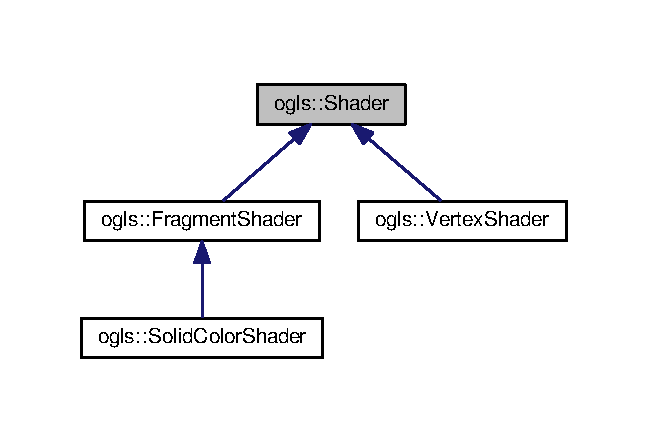
\includegraphics[width=312pt]{de/dba/classogls_1_1Shader__inherit__graph}
\end{center}
\end{figure}
\subsection*{Public Member Functions}
\begin{DoxyCompactItemize}
\item 
\hyperlink{classogls_1_1Shader_ac7b2a580207cd2ad1816cba87d40cc3a}{Shader} (G\-Lenum shader\-Type)
\begin{DoxyCompactList}\small\item\em \hyperlink{classogls_1_1Shader}{Shader} creates a new shader object of a given type. \end{DoxyCompactList}\item 
\hypertarget{classogls_1_1Shader_a9b5b5ec13be60e26176f334f30c112bc}{G\-Lenum {\bfseries type} ()}\label{classogls_1_1Shader_a9b5b5ec13be60e26176f334f30c112bc}

\item 
\hypertarget{classogls_1_1Shader_addde16b272f54d6de49b613f86fb409f}{\hyperlink{classogls_1_1Shader}{Shader} \& {\bfseries add\-Source} (std\-::istream \&stream)}\label{classogls_1_1Shader_addde16b272f54d6de49b613f86fb409f}

\item 
\hypertarget{classogls_1_1Shader_aa36972c2b14eb097b4bd0fd668ba60df}{\hyperlink{classogls_1_1Shader}{Shader} \& {\bfseries add\-Source} (std\-::string source)}\label{classogls_1_1Shader_aa36972c2b14eb097b4bd0fd668ba60df}

\item 
\hypertarget{classogls_1_1Shader_aee621433b4ced68bd9e801e5046884f1}{\hyperlink{classogls_1_1Shader}{Shader} \& {\bfseries compile} ()}\label{classogls_1_1Shader_aee621433b4ced68bd9e801e5046884f1}

\item 
\hypertarget{classogls_1_1Shader_adfce40703b571145882fcc1538316c8a}{\hyperlink{classogls_1_1Shader}{Shader} \& {\bfseries set\-Version} (short major, short minor)}\label{classogls_1_1Shader_adfce40703b571145882fcc1538316c8a}

\end{DoxyCompactItemize}


\subsection{Constructor \& Destructor Documentation}
\hypertarget{classogls_1_1Shader_ac7b2a580207cd2ad1816cba87d40cc3a}{\index{ogls\-::\-Shader@{ogls\-::\-Shader}!Shader@{Shader}}
\index{Shader@{Shader}!ogls::Shader@{ogls\-::\-Shader}}
\subsubsection[{Shader}]{\setlength{\rightskip}{0pt plus 5cm}Shader\-::\-Shader (
\begin{DoxyParamCaption}
\item[{G\-Lenum}]{shader\-Type}
\end{DoxyParamCaption}
)}}\label{classogls_1_1Shader_ac7b2a580207cd2ad1816cba87d40cc3a}


\hyperlink{classogls_1_1Shader}{Shader} creates a new shader object of a given type. 

Valid types are G\-L\-\_\-\-V\-E\-R\-T\-E\-X\-\_\-\-S\-H\-A\-D\-E\-R and G\-L\-\_\-\-F\-R\-A\-G\-M\-E\-N\-T\-\_\-\-S\-H\-A\-D\-E\-R.

If unsuccessful it will throw an \hyperlink{structogls_1_1ShaderException}{Shader\-Exception}


\begin{DoxyParams}{Parameters}
{\em shader\-Type} & the type of shader \\
\hline
\end{DoxyParams}
\begin{DoxySeeAlso}{See Also}
Vertex\-Shader(), Fragment\-Shader() 
\end{DoxySeeAlso}


The documentation for this class was generated from the following files\-:\begin{DoxyCompactItemize}
\item 
include/shader.\-hpp\item 
src/shader.\-cpp\end{DoxyCompactItemize}

\hypertarget{structogls_1_1ShaderException}{\section{ogls\-:\-:Shader\-Exception Struct Reference}
\label{structogls_1_1ShaderException}\index{ogls\-::\-Shader\-Exception@{ogls\-::\-Shader\-Exception}}
}


Inheritance diagram for ogls\-:\-:Shader\-Exception\-:
\nopagebreak
\begin{figure}[H]
\begin{center}
\leavevmode
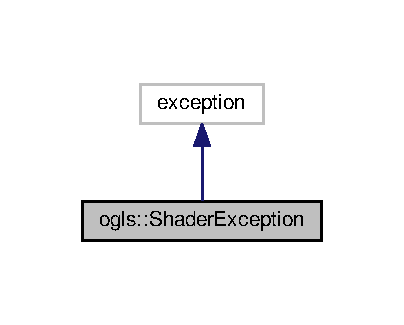
\includegraphics[width=194pt]{d5/dc9/structogls_1_1ShaderException__inherit__graph}
\end{center}
\end{figure}


Collaboration diagram for ogls\-:\-:Shader\-Exception\-:
\nopagebreak
\begin{figure}[H]
\begin{center}
\leavevmode
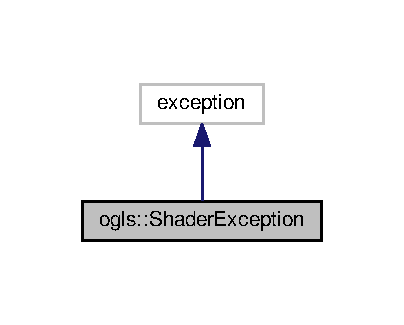
\includegraphics[width=194pt]{d1/df5/structogls_1_1ShaderException__coll__graph}
\end{center}
\end{figure}
\subsection*{Public Member Functions}
\begin{DoxyCompactItemize}
\item 
\hypertarget{structogls_1_1ShaderException_a0201786b9f03cf8d8c3314b6eb5fbee4}{{\bfseries Shader\-Exception} (std\-::string err)}\label{structogls_1_1ShaderException_a0201786b9f03cf8d8c3314b6eb5fbee4}

\item 
\hypertarget{structogls_1_1ShaderException_a021ae822f6a2d0e5105c4f9038275cf0}{const char $\ast$ {\bfseries what} () const   throw ()}\label{structogls_1_1ShaderException_a021ae822f6a2d0e5105c4f9038275cf0}

\end{DoxyCompactItemize}
\subsection*{Public Attributes}
\begin{DoxyCompactItemize}
\item 
\hypertarget{structogls_1_1ShaderException_a02ae515c005ead357aecbd109d1c97fd}{std\-::string {\bfseries m\-\_\-err}}\label{structogls_1_1ShaderException_a02ae515c005ead357aecbd109d1c97fd}

\end{DoxyCompactItemize}


The documentation for this struct was generated from the following file\-:\begin{DoxyCompactItemize}
\item 
include/shader.\-hpp\end{DoxyCompactItemize}

\hypertarget{classogls_1_1SolidColorShader}{\section{ogls\-:\-:Solid\-Color\-Shader Class Reference}
\label{classogls_1_1SolidColorShader}\index{ogls\-::\-Solid\-Color\-Shader@{ogls\-::\-Solid\-Color\-Shader}}
}


Inheritance diagram for ogls\-:\-:Solid\-Color\-Shader\-:\nopagebreak
\begin{figure}[H]
\begin{center}
\leavevmode
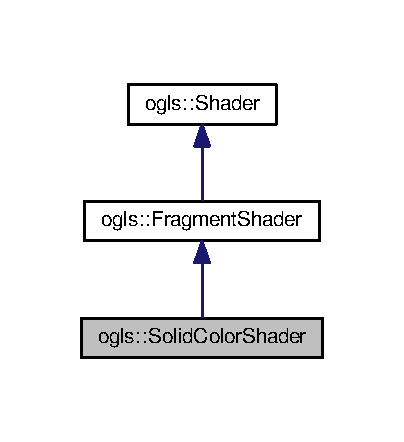
\includegraphics[width=194pt]{d0/d03/classogls_1_1SolidColorShader__inherit__graph}
\end{center}
\end{figure}


Collaboration diagram for ogls\-:\-:Solid\-Color\-Shader\-:\nopagebreak
\begin{figure}[H]
\begin{center}
\leavevmode
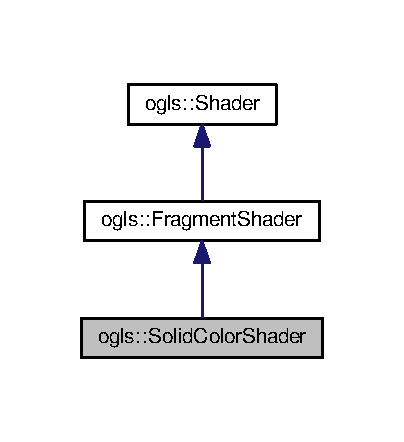
\includegraphics[width=194pt]{d7/d13/classogls_1_1SolidColorShader__coll__graph}
\end{center}
\end{figure}
\subsection*{Public Member Functions}
\begin{DoxyCompactItemize}
\item 
\hypertarget{classogls_1_1SolidColorShader_a7b87d06986b83421c7526e3a6f02f516}{{\bfseries Solid\-Color\-Shader} (\hyperlink{structogls_1_1ColorRGB}{Color\-R\-G\-B} color)}\label{classogls_1_1SolidColorShader_a7b87d06986b83421c7526e3a6f02f516}

\item 
\hypertarget{classogls_1_1SolidColorShader_afd557da82fc23157b9cbb07157f4fae2}{{\bfseries Solid\-Color\-Shader} (Color color)}\label{classogls_1_1SolidColorShader_afd557da82fc23157b9cbb07157f4fae2}

\item 
\hypertarget{classogls_1_1SolidColorShader_adaab2809e87c38d8233c2537bd15b503}{\hyperlink{structogls_1_1ColorRGB}{Color\-R\-G\-B} {\bfseries color} ()}\label{classogls_1_1SolidColorShader_adaab2809e87c38d8233c2537bd15b503}

\end{DoxyCompactItemize}


The documentation for this class was generated from the following files\-:\begin{DoxyCompactItemize}
\item 
include/shader.\-hpp\item 
src/shader.\-cpp\end{DoxyCompactItemize}

\hypertarget{classogls_1_1VertexShader}{\section{ogls\-:\-:Vertex\-Shader Class Reference}
\label{classogls_1_1VertexShader}\index{ogls\-::\-Vertex\-Shader@{ogls\-::\-Vertex\-Shader}}
}


Inheritance diagram for ogls\-:\-:Vertex\-Shader\-:
\nopagebreak
\begin{figure}[H]
\begin{center}
\leavevmode
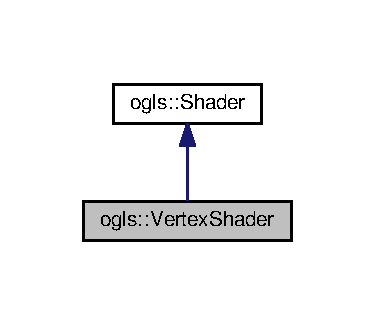
\includegraphics[width=180pt]{df/d56/classogls_1_1VertexShader__inherit__graph}
\end{center}
\end{figure}


Collaboration diagram for ogls\-:\-:Vertex\-Shader\-:
\nopagebreak
\begin{figure}[H]
\begin{center}
\leavevmode
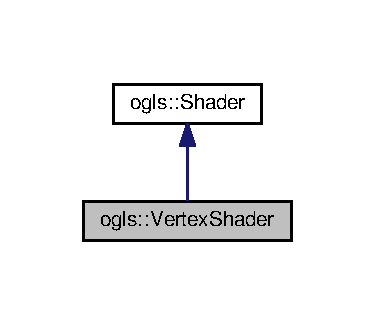
\includegraphics[width=180pt]{d3/d62/classogls_1_1VertexShader__coll__graph}
\end{center}
\end{figure}
\subsection*{Public Member Functions}
\begin{DoxyCompactItemize}
\item 
\hypertarget{classogls_1_1VertexShader_aed076b75f98fef94a264f3523a68c603}{{\bfseries Vertex\-Shader} (std\-::string source)}\label{classogls_1_1VertexShader_aed076b75f98fef94a264f3523a68c603}

\end{DoxyCompactItemize}


The documentation for this class was generated from the following files\-:\begin{DoxyCompactItemize}
\item 
include/shader.\-hpp\item 
src/shader.\-cpp\end{DoxyCompactItemize}

%--- End generated contents ---

% Index
\newpage
\phantomsection
\addcontentsline{toc}{chapter}{Index}
\printindex

\end{document}
